\documentclass{article}

\usepackage{graphicx}
\usepackage{tikz}
\usepackage{tikzsymbols}
\usetikzlibrary{calc,patterns,shapes.geometric}
\pagestyle{empty}
\usepackage[margin=0pt]{geometry}
\geometry{papersize={14in,12in}}

\def\centerarc[#1](#2)(#3:#4:#5){\draw[#1] ($(#2)+({#5*cos(#3)},{#5*sin(#3)})$) arc (#3:#4:#5);}

\begin{document}
	\begin{figure}
		\centering
		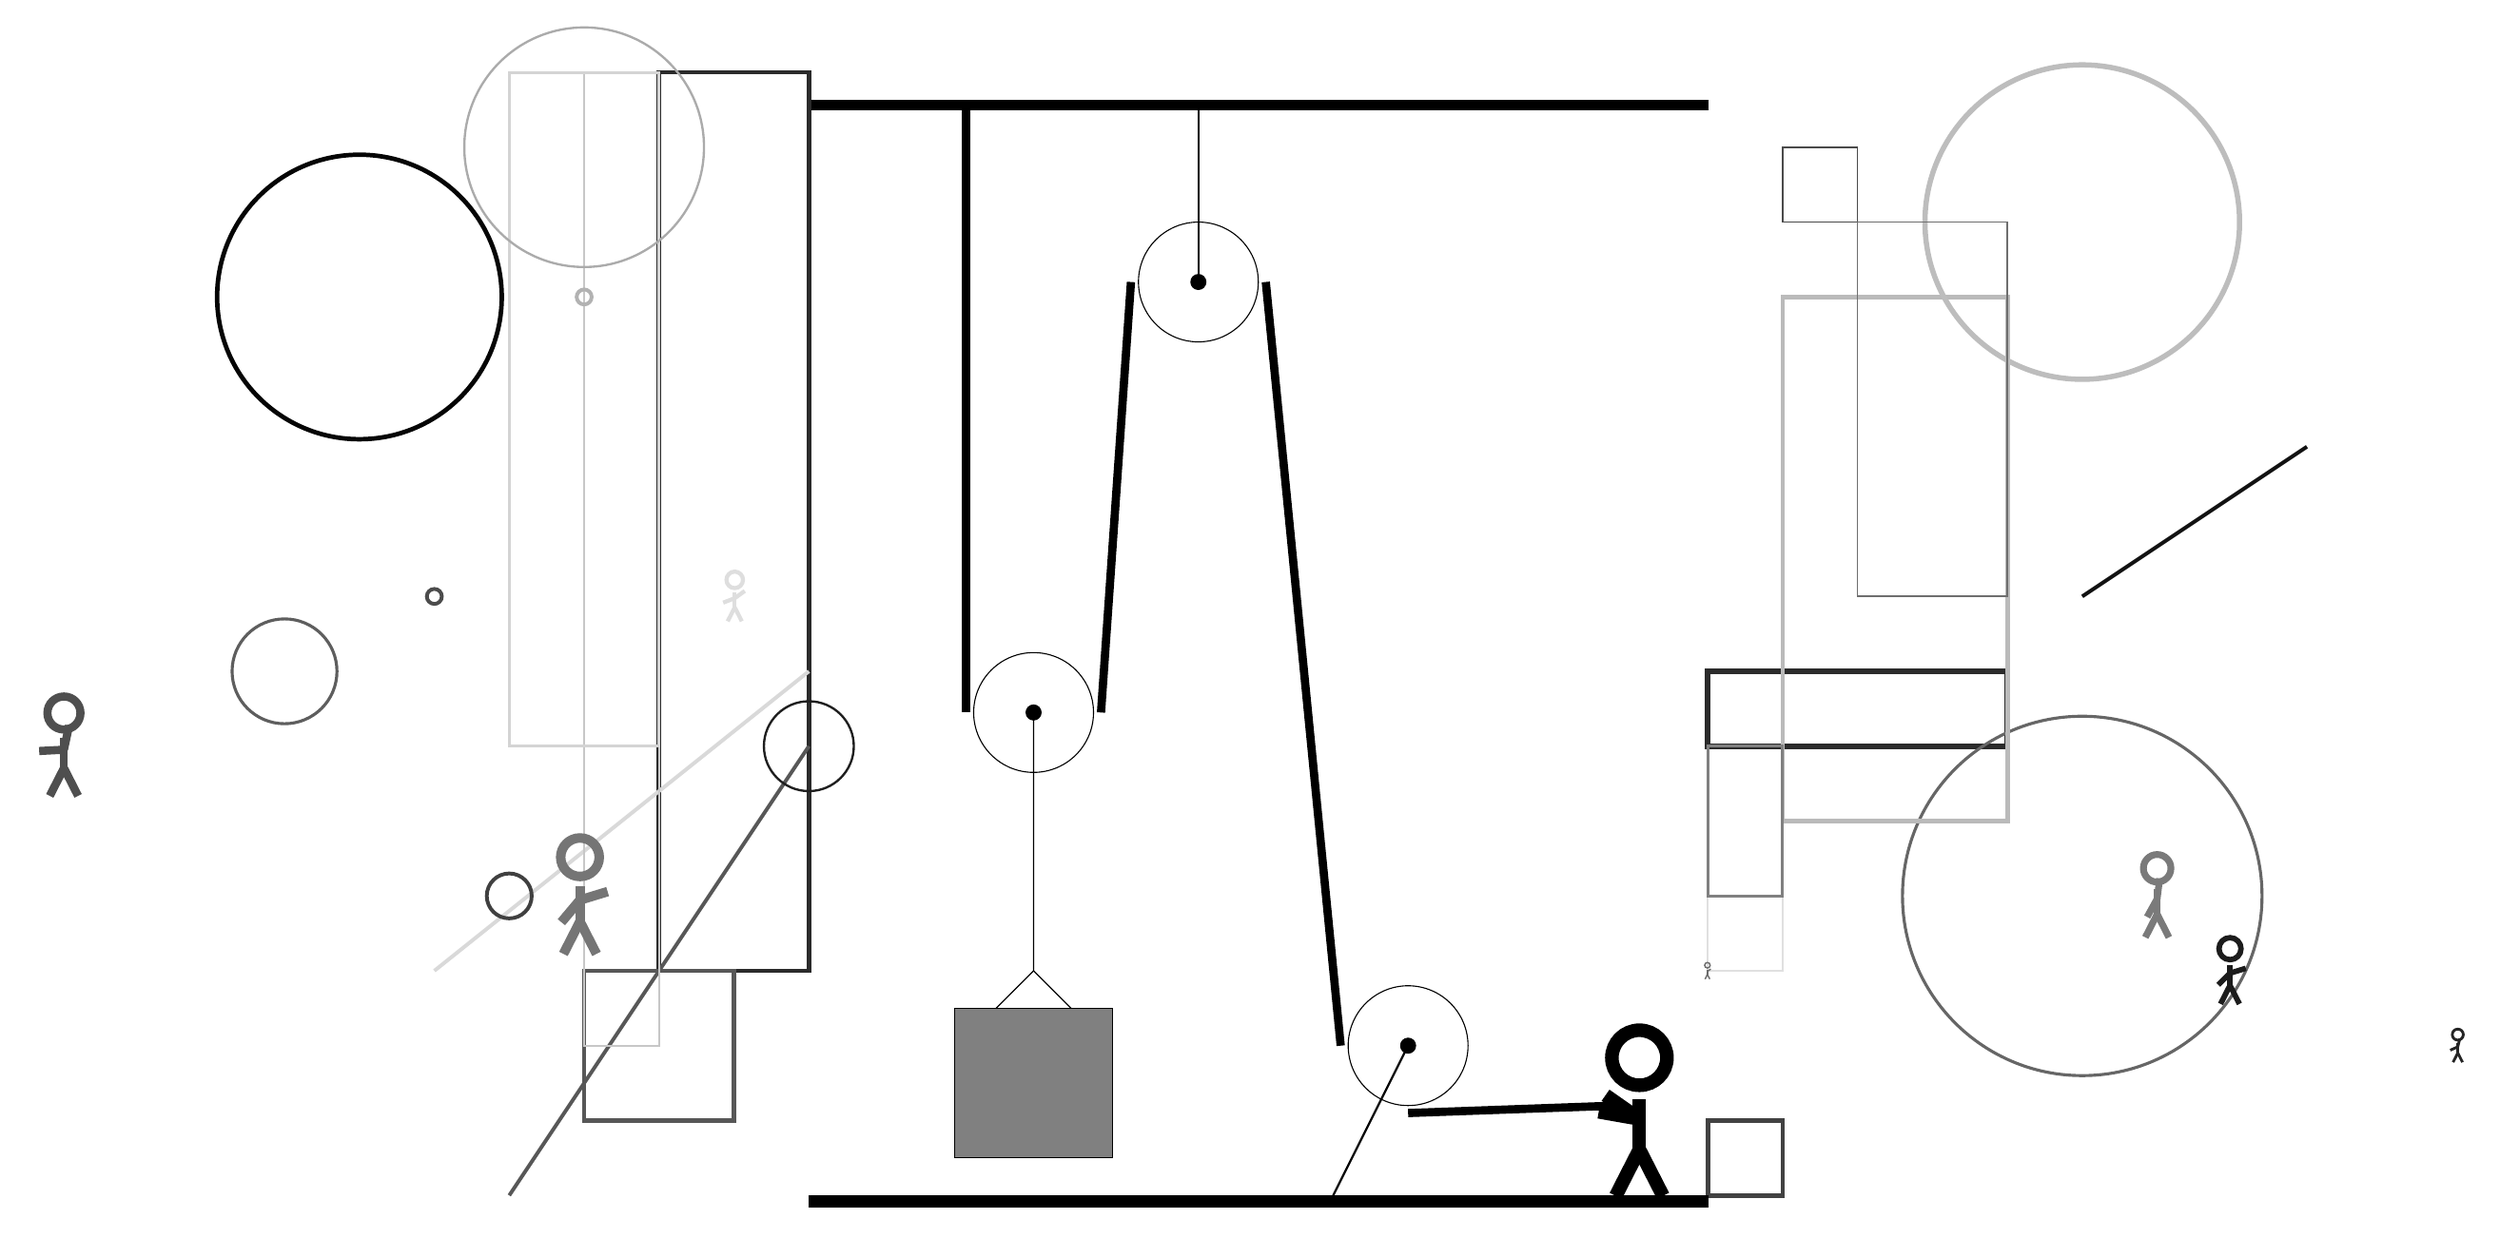
\begin{tikzpicture}
			%%%%% START %%%%%
			
			\draw[fill=black] (-2, 11.5) rectangle (10, 11.625);
			
			\draw (3.2, 9.2) circle (0.8);
			\draw[fill=black] (3.2, 9.2) circle (0.1);
			\draw[thick] (3.2, 9.2) -- (3.2, 11.5);
			
			\draw (6, -1) circle (0.8);
			\draw[fill=black] (6, -1) circle (0.1);
			\draw[thick] (6, -1) -- (5, -3);
			
			\draw (1, 3.45) circle (0.8);
			\draw[fill=black] (1, 3.45) circle (0.1);
			
			\draw (1, 3.45) -- (1, 0.0) -- (0.5, -0.5);
			\draw (1, 0.0) -- (1.5, -0.5);
			\draw[fill=black!50] (-0.05, -0.5) rectangle (2.05, -2.5);
			
			\draw[line width=1.1mm] (0.1, 11.5) -- (0.1, 3.45);
			\centerarc[line width=1.1mm](1, 3.45)(180:360:0.9);
			\draw[line width=1.1mm](1.9, 3.45) -- (2.3, 9.2);
			\centerarc[line width=1.1mm](3.2, 9.2)(0:180:0.9);
			\draw[line width=1.1mm](4.1, 9.2) -- (5.1, -1);
			\centerarc[line width=1.1mm](6, -1)(180:270:0.9);
			\draw[line width=1.1mm](6, -1.9) -- (8.8, -1.8);
			
			\draw[line width=0.7mm, color=black!83] (10, 3) rectangle (14, 4);
			
			\draw[line width=0.6mm, color=black!83] (-2, 0) rectangle (-4, 12);
			\draw[line width=0.6mm, color=black!66] (-3, -2) rectangle (-5, 0);
			\draw [line width=0.4mm, color=black!63](-9, 4) circle (0.7);
			\draw[line width=0.5mm, color=black!15](-2, 4) -- (-7, 0);
			\draw[line width=0.5mm, color=black!66](-6, -3) -- (-2, 3);
			\draw[line width=0.3mm, color=black!22] (-4, 12) rectangle (-5, -1);
			\node[line width=0.4mm, color=black!52] at (16, 1) {\Strichmaxerl[5][61][83]};
			\draw [line width=0.3mm, color=black!88](-2, 3) circle (0.6);
			\draw [line width=0.5mm, color=black!30](-5, 9) circle (0.1);
			\node[line width=0.4mm, color=black!69] at (-12, 3) {\Strichmaxerl[6][3][78]};
			
			\draw [line width=0.4mm, color=black!60](15, 1) circle (2.4);
			\draw[line width=0.4mm, color=black!17] (-4, 3) rectangle (-6, 12);
			\draw[line width=0.2mm, color=black!71] (12, 11) rectangle (11, 10);
			\draw [line width=0.3mm, color=black!33](-5, 11) circle (1.6);
			\draw [line width=0.6mm, color=black!98](-8, 9) circle (1.9);
			
			\draw[line width=0.6mm, color=black!74] (11, -3) rectangle (10, -2);
			
			\draw[line width=0.5mm, color=black!93](15, 5) -- (18, 7);
			\draw[line width=0.6mm, color=black!27] (11, 9) rectangle (14, 2);
			\draw [line width=0.5mm, color=black!70](-7, 5) circle (0.1);
			\node[line width=0.4mm, color=black!54] at (-5, 1) {\Strichmaxerl[7][50][17]};
			
			\node[line width=0.7mm, color=black!13] at (-3, 5) {\Strichmaxerl[3][21][36]};
			\draw [line width=0.5mm, color=black!75](-6, 1) circle (0.3);
			\draw[line width=0.3mm, color=black!12] (10, 1) rectangle (11, 0);
			\draw [line width=0.7mm, color=black!26](15, 10) circle (2.1);
			\draw[line width=0.4mm, color=black!50] (10, 3) rectangle (11, 1);
			\node[line width=0.7mm, color=black!89] at (17, 0) {\Strichmaxerl[4][45][17]};
			\draw[line width=0.2mm, color=black!57] (12, 10) rectangle (14, 5);
			\node[line width=0.7mm, color=black!58] at (10, 0) {\Strichmaxerl[1][86][35]};
			
			\node[line width=0.4mm, color=black!86] at (20, -1) {\Strichmaxerl[2][24][76]};
			
			\node at (9, -1.9) {\Strichmaxerl[10][-35][170]};
			
			\draw[fill=black] (-2, -3) rectangle (10, -3.15);
			
			%%%%% END %%%%%
		\end{tikzpicture}
	\end{figure}	
\end{document}